\begin{figure}[b]
\centering
\vspace{-6pt}
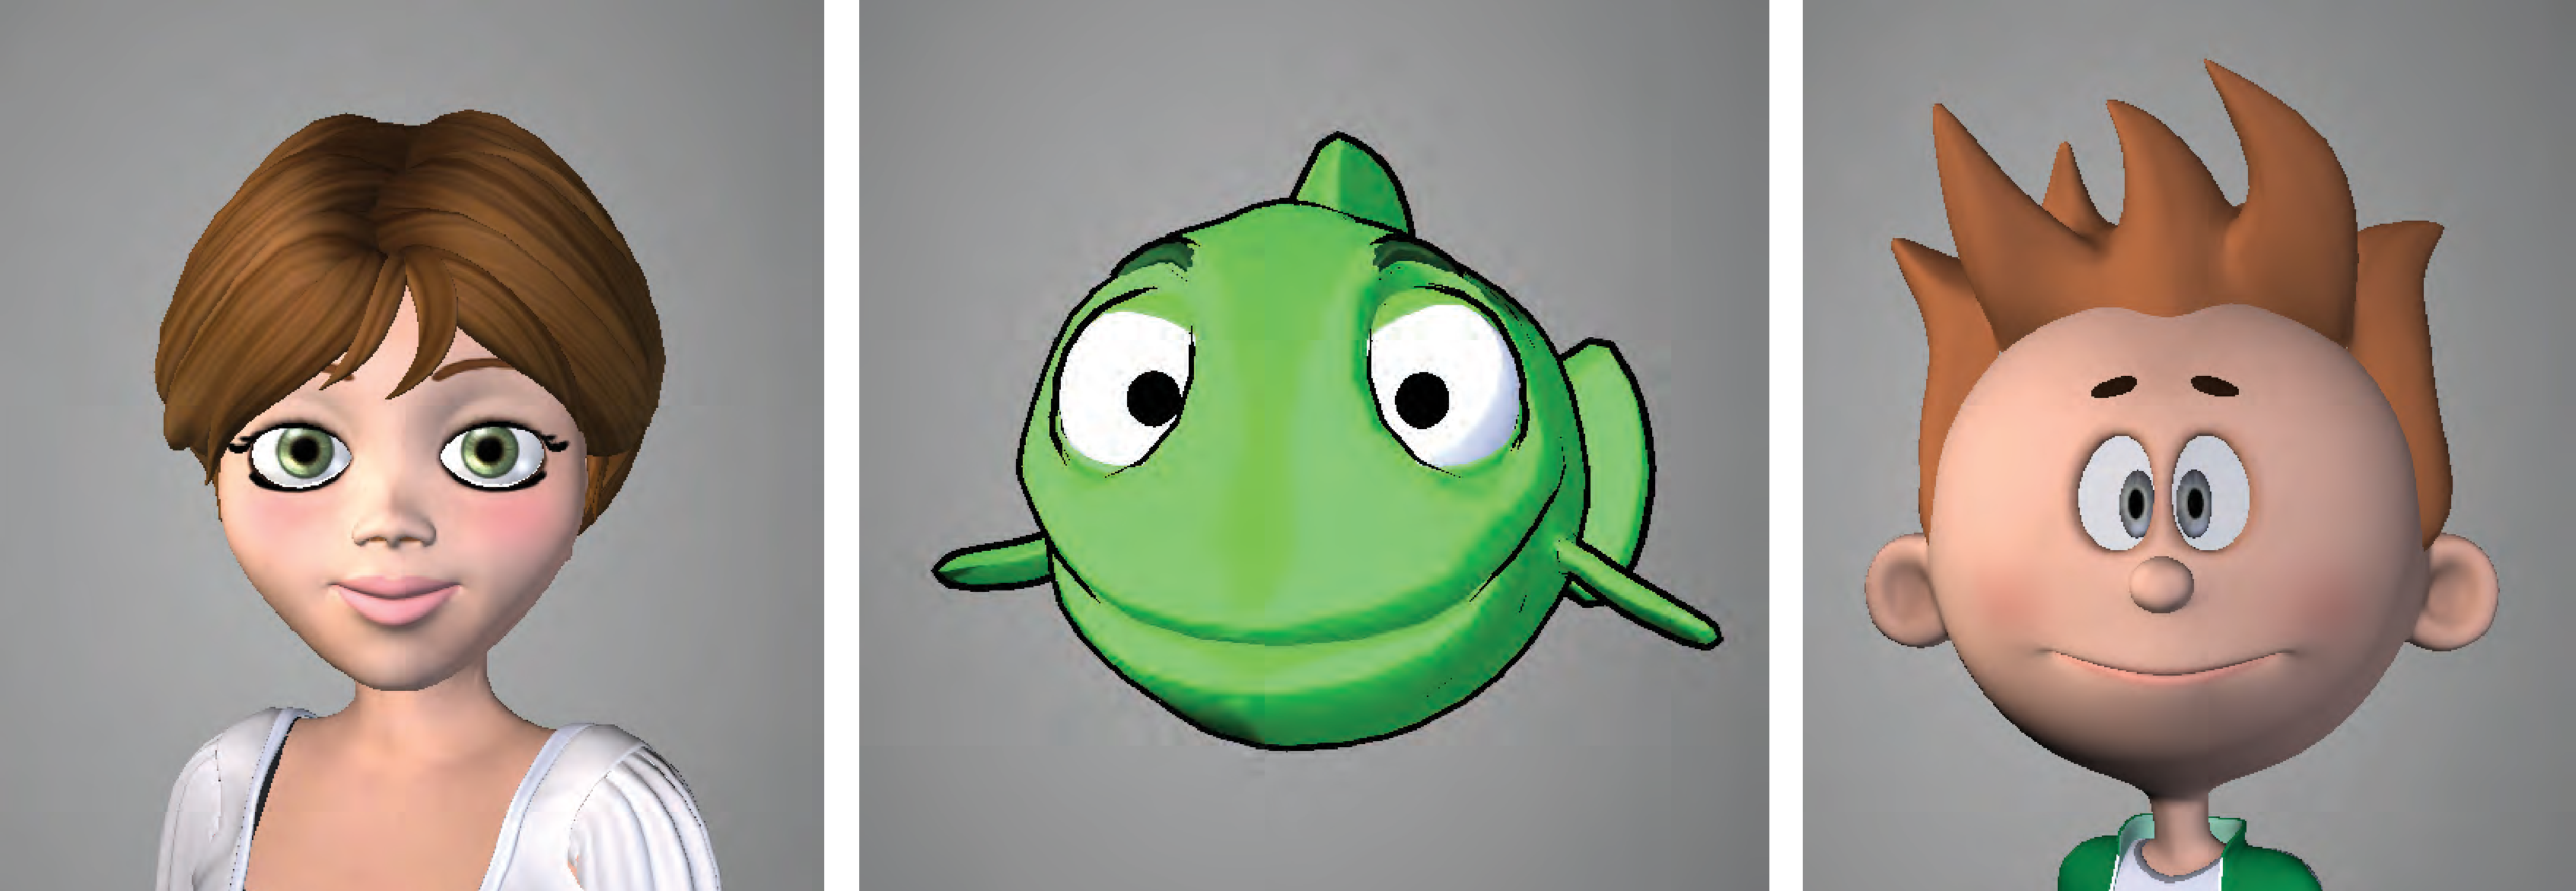
\includegraphics[width=0.48\textwidth]{Figures/StylizedCharacterExamples-small.pdf}
\caption{Examples of stylized characters. Characters 1 and 2 have large eyes and high inter-eye distance. Characters 2 and 3 have asymmetric eye motor range (OMR). Character 3 has narrow OMR and low inter-eye distance.}
\vspace{-6pt}
\label{fig:StylizedCharacterExamples}
\end{figure}

Gaze shifts are movements of the eyes and the head that redirect the gaze of a source toward a specific target. Animating gaze shifts for virtual humans often involves the use of parametric models of human gaze behavior. While these models enable virtual humans to perform natural and accurate gaze shifts, their use involves two key challenges. First, to capture the subtlety, richness, and expression of these movements, state-of-the-art models (e.g., \cite{andrist2012headeye,lance2010expressive}) incorporate anatomic and neurophysiological constraints as well as functional requirements. While these constraints enable characters that conform to the proportions of human anatomy to achieve humanlike gaze motion, they limit the applicability of these models to non-human or stylized characters. Such characters have exaggerated geometry with large and often asymmetrically shaped eyes such as those illustrated in Figure~\ref{fig:StylizedCharacterExamples}. Applying models of realistic human gaze motion to such characters can magnify or distort elements of gaze mechanics and potentially lead to anomalous poses and movements such as noticeable cross-eyedness or disconjugate eye movements. These phenomena can appear unpleasant and alter what these movements communicate.

Second, existing models seek to conform to functional constraints; the eyes must align with their target so that the character can see it. However, this requirement does not exist in theater, film, and cartoon animation, where the primary purpose of gaze shifts is to communicate ideas to the audience. For example, a stage actor does not need to physically align his eyes with an object of interest but merely needs to gaze toward the object's general direction to communicate his interest. Existing models lack support for animating such performative gaze behaviors.

To address these challenges, we present a model for \textit{stylized} and \textit{performative} gaze shifts that enhances a state-of-the-art model by relaxing model constraints in order to provide greater parametric control and applicability to a wider range of character designs. Stylized gaze shifts are enabled by a set of parameters for  character geometry (e.g., eye size and motor range) that adapt the target pose and gaze shift dynamics to the character's specific features. These extensions are designed to remain as faithful as possible to the human model while reducing undesirable artifacts.

Our model supports \textit{performative} gaze by relaxing the functional requirements and allowing explicit control over the degree of alignment with the viewer toward achieving greater social expressivity \cite{argyle1976gaze,goldberg1969distance,andrist2012designing}. The model also integrates \textit{view dependence}, which purposefully alters gaze direction (e.g., to remove cross-eyedness or achieve more alignment with the viewer) under the assumption that these alterations will not impair the viewer's perception of gaze direction. Prior studies of gaze indicate that observers can accurately identify face-directed gaze when the gaze source is facing them and otherwise use rough estimates of gaze direction based on head orientation \cite{cranach1973looking}. Informed by these findings, view dependency enables more flexible transformations of gaze direction when the character does not gaze directly at the viewer.

In order to animate gaze shifts in characters with a broader range of geometric properties while reducing artifacts and supporting performative gaze motion, our model departs from a validated model of human gaze behavior. An evaluation of the model confirms that it significantly reduces the frequency and severity of gaze artifacts across a wide range of characters and maintains the perceived naturalness and communicative accuracy of the state-of-the-art model.

The main contribution of this paper is a model for gaze shifts that applies to a wide range of characters and allows for performative effects. Specific contributions include:

\begin{itemize}
\item Identification of undesirable visual artifacts of models for human gaze behavior on stylized characters.
\item A model that incorporates parameters for character geometry and gaze dynamics into a model of human gaze behavior and allows animation of gaze motion for stylized characters with reduced visual artifacts.
\item An explicit consideration of performative gaze as part of a model, relaxing functional constraints where appropriate.
\end{itemize}